%%%%%%%%%%%%%%%%%%%%%%%%%%%%%%%%%%%%%%%%%
% Masters/Doctoral Thesis 
% LaTeX Template
% Version 2.5 (27/8/17)
%
% This template was downloaded from:
% http://www.LaTeXTemplates.com
%
% Version 2.x major modifications by:
% Vel (vel@latextemplates.com)
%
% This template is based on a template by:
% Steve Gunn (http://users.ecs.soton.ac.uk/srg/softwaretools/document/templates/)
% Sunil Patel (http://www.sunilpatel.co.uk/thesis-template/)
%
% Template license:
% CC BY-NC-SA 3.0 (http://creativecommons.org/licenses/by-nc-sa/3.0/)
%
%%%%%%%%%%%%%%%%%%%%%%%%%%%%%%%%%%%%%%%%%

%----------------------------------------------------------------------------------------
%	PACKAGES AND OTHER DOCUMENT CONFIGURATIONS
%----------------------------------------------------------------------------------------

\documentclass[
11pt, % The default document font size, options: 10pt, 11pt, 12pt
oneside, % Two side (alternating margins) for binding by default, uncomment to switch to one side
ngerman, % ngerman for German, english for English
singlespacing, % Single line spacing, alternatives: onehalfspacing or doublespacing
%draft, % Uncomment to enable draft mode (no pictures, no links, overfull hboxes indicated)
%nolistspacing, % If the document is onehalfspacing or doublespacing, uncomment this to set spacing in lists to single
%liststotoc, % Uncomment to add the list of figures/tables/etc to the table of contents
%toctotoc, % Uncomment to add the main table of contents to the table of contents
%parskip, % Uncomment to add space between paragraphs
%nohyperref, % Uncomment to not load the hyperref package
headsepline, % Uncomment to get a line under the header
chapterinoneline, % Uncomment to place the chapter title next to the number on one line
% consistentlayout, % Uncomment to change the layout of the declaration, abstract and acknowledgements pages to match the default layout
]{MastersDoctoralThesis} % The class file specifying the document structure

\usepackage[utf8]{inputenc} % Required for inputting international characters
\usepackage[T1]{fontenc} % Output font encoding for international characters

\usepackage{mathpazo} % Use the Palatino font by default

\usepackage[backend=bibtex,style=authoryear,natbib=true]{biblatex} % Use the bibtex backend with the authoryear citation style (which resembles APA)

% \addbibresource{example.bib} % The filename of the bibliography
\addbibresource{zotero.bib} % The filename of the bibliography

\usepackage[autostyle=true]{csquotes} % Required to generate language-dependent quotes in the bibliography

\usepackage{hyperref}
\usepackage{listings}

%----------------------------------------------------------------------------------------
%	MARGIN SETTINGS
%----------------------------------------------------------------------------------------

\geometry{
	paper=a4paper, % Change to letterpaper for US letter
	inner=2.5cm, % Inner margin
	outer=3.8cm, % Outer margin
	bindingoffset=.5cm, % Binding offset
	top=1.5cm, % Top margin
	bottom=1.5cm, % Bottom margin
	%showframe, % Uncomment to show how the type block is set on the page
}

%----------------------------------------------------------------------------------------
%	LISTING SETTINGS
%----------------------------------------------------------------------------------------

\lstdefinestyle{mystyle}{
    captionpos=b,
    numbers=left,
    numbersep=5pt,
    showspaces=false,
    showstringspaces=false,
    showtabs=false,
    tabsize=2
}
\lstset{style=mystyle}

%----------------------------------------------------------------------------------------
%	THESIS INFORMATION
%----------------------------------------------------------------------------------------

\thesistitle{Accessibility WID Dokumentation} % Your thesis title, this is used in the title and abstract, print it elsewhere with \ttitle
\supervisor{Rolf \textsc{Kruse}} % Your supervisor's name, this is used in the title page, print it elsewhere with \supname
\examiner{} % Your examiner's name, this is not currently used anywhere in the template, print it elsewhere with \examname
\degree{WID} % Your degree name, this is used in the title page and abstract, print it elsewhere with \degreename
\author{Tom \textsc{Käppler}} % Your name, this is used in the title page and abstract, print it elsewhere with \authorname
\addresses{} % Your address, this is not currently used anywhere in the template, print it elsewhere with \addressname

\subject{Web und Interaktions Design} % Your subject area, this is not currently used anywhere in the template, print it elsewhere with \subjectname
\keywords{} % Keywords for your thesis, this is not currently used anywhere in the template, print it elsewhere with \keywordnames
\university{\href{https://www.fh-erfurt.de/}{Fachhochschule Erfurt}} % Your university's name and URL, this is used in the title page and abstract, print it elsewhere with \univname
\department{\href{https://www.fh-erfurt.de/}{Department or School Name}} % Your department's name and URL, this is used in the title page and abstract, print it elsewhere with \deptname
\group{\href{http://researchgroup.university.com}{Research Group Name}} % Your research group's name and URL, this is used in the title page, print it elsewhere with \groupname
\faculty{\href{https://www.ai.fh-erfurt.de/}{Angewandte Informatik}} % Your faculty's name and URL, this is used in the title page and abstract, print it elsewhere with \facname

\AtBeginDocument{
\hypersetup{pdftitle=\ttitle} % Set the PDF's title to your title
\hypersetup{pdfauthor=\authorname} % Set the PDF's author to your name
\hypersetup{pdfkeywords=\keywordnames} % Set the PDF's keywords to your keywords
}

\begin{document}

\frontmatter % Use roman page numbering style (i, ii, iii, iv...) for the pre-content pages

\pagestyle{plain} % Default to the plain heading style until the thesis style is called for the body content

%----------------------------------------------------------------------------------------
%	TITLE PAGE
%----------------------------------------------------------------------------------------

\begin{titlepage}
\begin{center}

\vspace*{.06\textheight}
{\scshape\LARGE \univname\par}\vspace{1.5cm} % University name
% \textsc{\Large Dokumentation}\\[0.5cm] % Thesis type

\HRule \\[0.4cm] % Horizontal line
{\huge \bfseries \ttitle\par}\vspace{0.4cm} % Thesis title
\HRule \\[1.5cm] % Horizontal line
 
\begin{minipage}[t]{0.4\textwidth}
\begin{flushleft} \large
\emph{Author:}\\
\href{http://github.com/TKSpectro}{\authorname} % Author name - remove the \href bracket to remove the link
\end{flushleft}
\end{minipage}
\begin{minipage}[t]{0.4\textwidth}
\begin{flushright} \large
\emph{Supervisor:} \\
\href{https://www.ai.fh-erfurt.de/kruse}{\supname} % Supervisor name - remove the \href bracket to remove the link  
\end{flushright}
\end{minipage}\\[3cm]
 
\vfill

% \large \textit{A thesis submitted in fulfillment of the requirements\\ for the degree of \degreename}\\[0.3cm] % University requirement text
% \textit{in the}\\[0.4cm]
% \groupname\\\deptname\\[2cm] % Research group name and department name
 
\vfill

{\large \today}\\[4cm] % Date
%\includegraphics{Logo} % University/department logo - uncomment to place it
 
\vfill
\end{center}
\end{titlepage}

%----------------------------------------------------------------------------------------
%	DECLARATION PAGE
%----------------------------------------------------------------------------------------

% \begin{declaration}
% \addchaptertocentry{\authorshipname} % Add the declaration to the table of contents
% \noindent I, \authorname, declare that this thesis titled, \enquote{\ttitle} and the work presented in it are my own. I confirm that:

% \begin{itemize} 
% \item This work was done wholly or mainly while in candidature for a research degree at this University.
% \item Where any part of this thesis has previously been submitted for a degree or any other qualification at this University or any other institution, this has been clearly stated.
% \item Where I have consulted the published work of others, this is always clearly attributed.
% \item Where I have quoted from the work of others, the source is always given. With the exception of such quotations, this thesis is entirely my own work.
% \item I have acknowledged all main sources of help.
% \item Where the thesis is based on work done by myself jointly with others, I have made clear exactly what was done by others and what I have contributed myself.\\
% \end{itemize}
 
% \noindent Signed:\\
% \rule[0.5em]{25em}{0.5pt} % This prints a line for the signature
 
% \noindent Date:\\
% \rule[0.5em]{25em}{0.5pt} % This prints a line to write the date
% \end{declaration}

% \cleardoublepage

%----------------------------------------------------------------------------------------
%	QUOTATION PAGE
%----------------------------------------------------------------------------------------

% \vspace*{0.2\textheight}

% \noindent\enquote{\itshape Thanks to my solid academic training, today I can write hundreds of words on virtually any topic without possessing a shred of information, which is how I got a good job in journalism.}\bigbreak

% \hfill Dave Barry

%----------------------------------------------------------------------------------------
%	ABSTRACT PAGE
%----------------------------------------------------------------------------------------

% \begin{abstract}
% \addchaptertocentry{\abstractname} % Add the abstract to the table of contents
% The Thesis Abstract is written here (and usually kept to just this page). The page is kept centered vertically so can expand into the blank space above the title too\ldots
% \end{abstract}

%----------------------------------------------------------------------------------------
%	ACKNOWLEDGEMENTS
%----------------------------------------------------------------------------------------

% \begin{acknowledgements}
% \addchaptertocentry{\acknowledgementname} % Add the acknowledgements to the table of contents
% The acknowledgments and the people to thank go here, don't forget to include your project advisor\ldots
% \end{acknowledgements}

%----------------------------------------------------------------------------------------
%	LIST OF CONTENTS/FIGURES/TABLES PAGES
%----------------------------------------------------------------------------------------

\tableofcontents % Prints the main table of contents

\listoffigures % Prints the list of figures

\listoftables % Prints the list of tables

%----------------------------------------------------------------------------------------
%	ABBREVIATIONS
%----------------------------------------------------------------------------------------

\begin{abbreviations}{ll} % Include a list of abbreviations (a table of two columns)

\textbf{WID} & \textbf{W}eb und \textbf{I}nteraction \textbf{D}esign\\
\textbf{a11y} & \textbf{A}ccessibilt\textbf{y}\\
\textbf{ARIA} & \textbf{A}ccessible \textbf{R}ich \textbf{I}nternet \textbf{A}pplications\\
\textbf{ARIA APG} & ARIA \textbf{A}uthoring \textbf{P}ractices \textbf{G}uide\\
\textbf{UI} & \textbf{U}ser \textbf{I}nterface\\
\textbf{GUI} & \textbf{G}raphical \textbf{U}ser \textbf{I}nterface\\

\end{abbreviations}

%----------------------------------------------------------------------------------------
%	PHYSICAL CONSTANTS/OTHER DEFINITIONS
%----------------------------------------------------------------------------------------

% \begin{constants}{lr@{${}={}$}l} % The list of physical constants is a three column table

% % The \SI{}{} command is provided by the siunitx package, see its documentation for instructions on how to use it

% Speed of Light & $c_{0}$ & \SI{2.99792458e8}{\meter\per\second} (exact)\\
% %Constant Name & $Symbol$ & $Constant Value$ with units\\

% \end{constants}

%----------------------------------------------------------------------------------------
%	SYMBOLS
%----------------------------------------------------------------------------------------

% \begin{symbols}{lll} % Include a list of Symbols (a three column table)

% $a$ & distance & \si{\meter} \\
% $P$ & power & \si{\watt} (\si{\joule\per\second}) \\
% %Symbol & Name & Unit \\

% \addlinespace % Gap to separate the Roman symbols from the Greek

% $\omega$ & angular frequency & \si{\radian} \\

% \end{symbols}

%----------------------------------------------------------------------------------------
%	DEDICATION
%----------------------------------------------------------------------------------------

% \dedicatory{For/Dedicated to/To my\ldots} 

%----------------------------------------------------------------------------------------
%	THESIS CONTENT - CHAPTERS
%----------------------------------------------------------------------------------------

\mainmatter % Begin numeric (1,2,3...) page numbering

\pagestyle{thesis} % Return the page headers back to the "thesis" style

% Include the chapters of the thesis as separate files from the Chapters folder
% Uncomment the lines as you write the chapters

\chapter{Einführung} 
\label{Introduction}

In den letzten Jahren hat die Bedeutung von Web-Accessibility, also der Zugänglichkeit von Webinhalten für Menschen mit Behinderungen, stark zugenommen. Das Internet bietet eine Vielzahl von Informationen und Dienstleistungen, die für Menschen mit eingeschränkten körperlichen oder geistigen Fähigkeiten von großer Bedeutung sind. Es ist daher von entscheidender Bedeutung, dass Web-Entwickler ihre Websites barrierefrei gestalten, um sicherzustellen, dass alle Benutzer sie problemlos nutzen können.

Zum Glück gibt es heute eine Vielzahl von Tools, die Entwicklern dabei helfen können, barrierefreie Websites zu erstellen. Diese reichen von einfachen Validierungs-Tools, die überprüfen, ob eine Website bestimmte Standards erfüllt, bis hin zu komplexen Werkzeugen, die sich speziell auf die Bedürfnisse von Menschen mit Behinderungen konzentrieren.

In dieser Ausarbeitung wird sich mit einigen der wichtigsten Tools und Techniken beschäftigen, die Entwicklern zur Verfügung stehen, um sicherzustellen, dass ihre Websites barrierefrei sind. Es wird sich unter anderem auch mit der Beispielhaften Umsetzung einer barrierefreien Website beschäftigt und anhand dieser verschiedene Techniken und Libraries vorgestellt.
\chapter{Zeitplan}

\label{Chapter2}

\begin{itemize}
    \item Ende November: Recherche, welche Libraries eingesetzt werden und anfangen diese einzubinden
    \item Ende Dezember: Website in der grundlegenden Form fertig
    \item Ende Januar: Mit verschiedenen Tools, verschiedene a11y Aspekte testen und dokumentieren
    \item Ende Februar: Website optimieren, dokumentieren und Tests mit den a11y Tools fertig
\end{itemize}
\chapter{Recherche}
\label{Research}

\section{Allgemeines}

Der Begriff \emph{Accessibility} oder abgekürzt \emph{a11y} bezeichnet eine Gestaltung der Umwelt, sodass sie auch von Menschen mit Beeinträchtigungen ohne zusätzliche Hilfen genutzt und wahrgenommen werden kann. \cite{bundesfachstelle_barrierefreiheit_wie_nodate} 

Zu diesen Beeinträchtigungen zählen unter anderem:

\begin{itemize}
    \item Auditiv
    \item Kognitiv
    \item Neurologisch
    \item Physisch
    \item Sprache
\end{itemize}

Die Umsetzung von a11y auf Webseiten kann außerdem bei temporären Einschränkungen helfen, wie z.B. bei einer Verletzung oder einer Krankheit, einem gebrochenen Arm oder einer verlorenen Brille. Ebenfalls kann es bei situationsabhängigen Limitierungen helfen, wie z.B. helles Tageslicht oder ein lauter Raum in dem ein Audio/Video nicht hörbar ist.

\section{ARIA Authoring Practices Guide (APG)}

Der ARIA Authoring Practices Guide kurz (APG) ist eine Sammlung von Beispielen und Best Practices für die Verwendung von ARIA. \cite{w3c_web_accessibility_initiative_wai_aria_nodate} Es werden verschiedene Themen wie z.B. Farbkontraste, Semantisches HTML, Fokus Kontroller und noch einiges mehr behandelt. Diese werden mit Beispielen und tiefgehenden Erklärungen dargestellt und an praktischen Beispielen erläutert.

\subsection{Patterns}
\label{secsec:apg_patterns}

Der Guide stellt für quasi alle Elemente die in einer normalen Webseite vorkommen, ein Pattern, also eine Beschreibung welche Dinge bachtet werden müssen, bereit. Dies fängt bei einfachen HTML-Elementen wie z.B. Buttons oder Links an und geht bis hin zu komplexeren Elementen wie z.B. Accordions, Carousels oder Dialogen (Modale). \cite{initiative_wai_patterns_nodate}

Für den Dialog wird z.B. ersteinmal grundlegend erklärt wie genau ein Dialog funktioniert und welche Elemente er beinhaltet. Danach wird auf die Tastatur Interaktionen eingegangen, welche implementiert werden sollten und auch welche HTML-Aria-Eigenschaften dafür genutzt werden können, um die best mögliche a11y zu gewährleisten. In dem direkt bereitgestellten Beispiel wird dann die Implementierung dieser Eigenschaften gezeigt und bis in kleinste Detail erläutert was jede einzelne davon bewirkt und warum diese genutzt wird.

\subsection{Landmark Regions}

Landmark Regions sind Bereiche einer Webseite, welche für Screenreader und andere Hilfsmittel wie z.B. Sprungmarken wichtig sind. \cite{initiative_wai_landmark_nodate} Diese werden in der Dokumentation mit Beispielen und Erklärungen vorgestellt und erklärt.

Zuerst wird auf die HTML Stuktur Elemente eingegangen. Dazu gehören z.B. \emph{<header>}, \emph{<main>}, \emph{<footer>} und \emph{<nav>}. Diese werden mit Beispielen und Erklärungen vorgestellt und erklärt. Danach wird auf die ARIA Eigenschaften eingegangen, welche für die Landmark Regions genutzt werden können. Diese sind z.B. \emph{role="banner"}, \emph{role="main"}, \emph{role="contentinfo"} und \emph{role="navigation"}. Mit diesen können bestimmte Bereiche oder Informationen für Screenreader und andere Hilfsmittel markiert werden.

\subsection{Accessible Names and Descriptions}

Accessible Names and Descriptions sind die Namen und Beschreibungen von Elementen, welche z.B. für Screenreader wichtig sind. \cite{initiative_wai_providing_nodate} In der Dokumentation wird ausführlichst darauf eingegangen wie genau man diese Namen und Beschreibungen aufbauen und vergeben sollte und welche Möglichkeiten es dafür gibt. Dies wird auch hier wieder durch eine vielzahl an Beispielen zu den verschiedenen Möglichkeiten unterstüzt.

Außerdem werden Grundregeln für die Namensgebung vorgestellt. Diese sind z.B.:

\begin{itemize}
    \item Beachtung von Warnungen und ausführliches Testen
    \item Sichtbaren Text bevorzugen
    \item Native Techniken bevorzugen (z.B. \emph{<label>})
    \item Browser Fallbacks vermeiden
    \item Kurze und nützliche Namen und Beschreibungen nutzen
\end{itemize}

\subsection{Keyboard Interface}

Damit eine Seite komplett und vorallem auch barrierefrei nur mit Hilfe einer Tastatur bedienbar ist, müssen einige Dinge beachtet und explizit implementiert werden. Dies muss passieren, da die meisten Browser, im Gegensatz zu nativen Form-Elementen, keinen direkten Tastatur Support für das Steuern von GUI Komponenten bieten. \cite{initiative_wai_developing_nodate} Dies muss z.B. für Menüs, Grids, Toolbars und Dialoge von den Entwicklern übernommen werden.

Die wichtigste und fundametalste Tastaturnavigation ist die Tabulator Navigation. Diese wird per \emph{Tab} und \emph{Shift + Tab} gesteuert und ermöglicht es den Fokus von einem UI Element auf das nächste zu bewegen. Zusätlich können dann die Pfeiltasten genutzt werden um den Fokus innerhalb einer Komponente zu bewegen. \cite{initiative_wai_developing_nodate}

Anschließend wird in der Dokumenation noch erweiternd auf die folgenden Themen eingegangen:

\begin{itemize}
    \item Erkennbarer und vorhersehbarer Tastaturfokus
    \item Fokus vs. Selektion und die Wahrnehmung eines doppelten Fokuses
    \item Wann sollte die Auswahl dem Fokus automatisch folgen
    \item Tastaturnavigation zwischen Komponenten (Die Tab-Sequence)
    \item Tastaturnavigation innerhalb von Komponenten
    \item Fokussierbarkeit von deaktivierten Steuerelementen
    \item Tastenzuweisungskonventionen für allgemeine Funktionen
    \item Tastaturkurzbefehle und wie diese vergeben werden sollten
\end{itemize}

\section{Tools zur Analyse}

Die folgenden Tools wurden in der Recherche gefunden und können zur Analyse von Webseiten verwendet werden. Eine ausführliche Beschreibung der einzelnen Tools findet sich in den jeweiligen Kapiteln.

\begin{itemize}
    \item \hyperref[sec:a11yToolsLighthouse]{Lighthouse (SEO, Performance, Accessibility Analyse)}
    \item \hyperref[sec:a11yToolsIBMEAAC]{IBM Equal Access Accessibility Checker}
    \item \hyperref[sec:a11yToolsAxe]{Deque Axe (Accessibility Analyse)}
    \item \hyperref[sec:a11yToolsWAVE]{Wave (Accessibility Analyse)}
    \item \hyperref[sec:a11yToolsJAWS]{JAWS (Screenreader)}
    \item \hyperref[sec:a11yToolsNVDA]{NVDA (Screenreader)}
\end{itemize}

\section{Storyook}

Storybook ist eine Open-Source-JavaScript-Bibliothek, die es Entwicklern ermöglicht, Komponenten isoliert und unabhängig voneinander zu entwickeln, zu testen und zu dokumentieren. \cite{storybook_storybook_nodate} Mit Storybook können Entwickler eine interaktive und benutzerfreundliche Benutzeroberfläche erstellen, um ihre Komponenten in verschiedenen Zuständen zu präsentieren, ohne dabei auf eine vollständige Anwendung angewiesen zu sein.

Storybook ist besonders nützlich für Projekte, die auf Komponentenarchitekturen und Design-Systemen basieren, da es Entwicklern hilft, Komponenten unabhängig voneinander zu testen und sicherzustellen, dass sie ordnungsgemäß funktionieren, bevor sie in die Anwendung integriert werden.

Die Bibliothek bietet außerdem verschiedene Add-Ons und Tools, die es Entwicklern ermöglichen, die Zugänglichkeit ihrer Komponenten zu überprüfen und sicherzustellen, dass sie die Anforderungen der Web Content Accessibility Guidelines (WCAG) erfüllen.

Ein Beispiel für ein Accessibility-Add-On in Storybook ist das a11y Add-On, das eine Integration mit der Accessibility Testing-Engine \hyperref[sec:a11yToolsAxe]{\emph{axe-core}} bietet. Mit diesem Add-On können Entwickler ihre Komponenten auf Barrierefreiheitsprobleme testen, wie z.B. fehlende Alternativtexte für Bilder oder mangelnde Kontrastverhältnisse für Texte und Hintergründe.

Ein weiteres Beispiel ist das \emph{Storybook Addon Docs} Add-On, das es Entwicklern ermöglicht, Dokumentationen für ihre Komponenten zu erstellen, einschließlich der Zugänglichkeitsanforderungen und -hinweise für jede Komponente.

Zusammenfassend bietet Storybook verschiedene Möglichkeiten, um die Zugänglichkeit von Komponenten zu testen und sicherzustellen, dass sie für alle Benutzer, einschließlich derjenigen mit Behinderungen, zugänglich sind.

\section{Angular}

\subsection{Material UI}

Angular Material UI (MUI) ist eine Sammlung von UI Komponenten, die auf Angular basieren. \cite{angular_components_team_angular_nodate} Diese sind teilweise bereits mit a11y ausgestattet, wie z.B. die \href{https://material.angular.io/components/select/overview#accessibility}{Selects} oder \href{https://material.angular.io/components/checkbox/overview#accessibility}{Checkboxen}. Neben den automatisch eingestellten ARIA-Tags gibt die Dokumentation für die meisten Komponenten weitere Tags an, welche vom Entwickler gesetzt werden sollten. Siehe z.B. \href{https://material.angular.io/components/dialog/overview#accessibility}{Dialog}.

MUI bietet außerdem ein \emph{Component Dev Kit (CDK)} an. Dieses bietet verschiedene Hilfsfunktionen, welche für die Entwicklung von eigenen a11y optimierten Komponenten verwendet werden können. \cite{angular_components_team_angular_nodate}

Die Vorteile von Material UI sind:

\begin{itemize}
    \item Zugänglichkeit: Material UI legt Wert auf Accessibility-Features und stellt sicher, dass alle Komponenten vollständig zugänglich sind, um eine barrierefreie Nutzung der Webanwendung zu gewährleisten.
    \item Leicht anpassbar: Material UI bietet eine Vielzahl von Möglichkeiten, um Komponenten an das Design der Anwendung anzupassen. Dabei können Themes, Farben und andere Design-Elemente einfach angepasst werden.
    \item Große Community: Material UI hat eine große Community von Entwicklern, die dazu beitragen, die Bibliothek ständig zu verbessern und zu erweitern.
\end{itemize}

Ein Nachteil ist, dass die Bibliothek möglicherweise nicht so gut anpassbar ist wie andere UI-Bibliotheken, insbesondere wenn es um das Layout geht. Dies kann zu Einschränkungen bei der Gestaltung von Webanwendungen führen. Bestimmte Stylings müssen über teilweise umstandliche CSS-Regeln angepasst werden und überschrieben werden.

Insgesamt ist Material UI eine robuste Bibliothek mit vielen nützlichen Funktionen und einem großen Unterstützungssystem. Es ist eine gute Wahl für Entwickler, die eine umfassende UI-Lösung für Angular suchen, besonders wenn Zugänglichkeit und Benutzerfreundlichkeit eine hohe Priorität haben.

\subsection{Google Codelab - Angular a11y}

Google Codelab sind Lernkurse zur eigenständigen Bearbeitung. In diesem Codelab wird ein Beispielprojekt erstellt, welches die Grundlagen von a11y in Angular beinhaltet. Dabei werden Themen wie z.B. Farbkontraste, Semantisches HTML, Fokus Kontroller und verschiedene andere Dinge behandlet.

\section{React}

\subsection{React-Aria}

React-Aria ist eine React-Bibliothek, die von Adobe entwickelt wurde und es Entwicklern ermöglicht, barrierefreie Benutzeroberflächen in React zu erstellen. Die Bibliothek bietet eine Sammlung von React-Komponenten und Hooks, die speziell für die Unterstützung von Accessibility-Funktionen entwickelt wurden.

Die Vorteile von React-Aria sind:

\begin{itemize}
    \item Accessibility-Features: React-Aria bietet Entwicklern eine einfache und konsistente Möglichkeit, Accessibility-Features wie Tastaturzugänglichkeit und Screen-Reader-Kompatibilität in ihre React-Komponenten zu integrieren.
    \item Einfachheit: React-Aria bietet eine einfache API und eine umfassende Dokumentation, die es Entwicklern erleichtert, barrierefreie Komponenten zu erstellen.
    \item Flexibilität: React-Aria bietet eine Vielzahl von Konfigurationsoptionen, um sicherzustellen, dass die Accessibility-Funktionen den Bedürfnissen des Benutzers entsprechen. Entwickler können z.B. die Reihenfolge der Fokusnavigation anpassen oder die Funktionsweise von ARIA-Attributen konfigurieren.
    \item Aktive Community: React-Aria hat eine aktive Entwickler-Community, die regelmäßig Updates und Verbesserungen zur Verfügung stellt und Fragen beantwortet.
\end{itemize}

Ein Nachteil von React-Aria ist, dass die Bibliothek möglicherweise nicht für alle Anwendungsfälle geeignet ist. Da die Accessibility-Funktionen von React-Aria zusätzliche Markup- und Code-Elemente erfordern, kann dies zu einer erhöhten Komplexität von React-Komponenten führen.

Ein weiterer möglicher Nachteil ist, dass Entwickler, die nicht vertraut sind mit den Accessibility-Features von React-Aria, eine zusätzliche Lernkurve haben können, um die Bibliothek effektiv einzusetzen.

\subsection{HeadlessUI}

HeadlessUI ist eine React-Bibliothek, die von Tailwind Labs entwickelt wurde und eine Sammlung von vollständig zugänglichen und wiederverwendbaren Headless-Komponenten bietet. HeadlessUI ist darauf ausgelegt, Entwicklern die Erstellung von benutzerdefinierten, zugänglichen Benutzeroberflächen zu erleichtern.

Die Vorteile von HeadlessUI sind:

\begin{itemize}
    \item Accessibility-Features: HeadlessUI-Komponenten sind vollständig zugänglich und unterstützen Tastaturzugänglichkeit, Screenreader-Unterstützung und andere Accessibility-Features, die die Barrierefreiheit von Webanwendungen verbessern.
    \item Anpassbarkeit: HeadlessUI-Komponenten sind \emph{headless}, d.h. sie haben keine vorgegebene visuelle Darstellung und können einfach an das Design der Anwendung angepasst werden.
    \item Einfache Integration: HeadlessUI kann nahtlos in bestehende React-Projekte integriert werden, da es nur minimale Abhängigkeiten hat und einfach zu verwenden ist.
    \item Gute Dokumentation: HeadlessUI bietet eine ausführliche Dokumentation und viele Beispiele, die Entwicklern helfen, die Bibliothek schnell und effektiv einzusetzen.
\end{itemize}

Ein möglicher Nachteil von HeadlessUI ist, dass die Bibliothek möglicherweise nicht für alle Anwendungsfälle geeignet ist. Da die Komponenten so anpassbar sind, erfordert ihre Verwendung möglicherweise mehr Code als die Verwendung von vorgefertigten UI-Komponenten.

Ein weiterer möglicher Nachteil ist, dass die Bibliothek noch relativ neu ist und möglicherweise nicht so gut etabliert und weit verbreitet wie einige andere UI Bibliotheken. Dies kann zu einer begrenzten Unterstützung von Drittanbietern und einer kleineren Entwickler-Community führen.

\subsection{Radix}
\label{secsec:radix}

Radix ist eine React-Bibliothek, die von Modulz entwickelt wurde und eine Sammlung von wiederverwendbaren Komponenten enthält, die auf einer \emph{primitive-first} Designphilosophie basieren. Radix stellt Komponenten zur Verfügung, die den Primitiven von HTML und CSS ähneln, um den Zugriff auf wichtige Accessibility-Features sicherzustellen.

Die Vorteile von Radix sind:

\begin{itemize}
    \item Accessibility-Features: Radix-Komponenten sind vollständig zugänglich und unterstützen Tastaturzugänglichkeit, Screenreader-Unterstützung und andere Accessibility-Features, die die Barrierefreiheit von Webanwendungen verbessern.
    \item Einfache Integration: Radix kann nahtlos in bestehende React-Projekte integriert werden, da es nur minimale Abhängigkeiten hat und einfach zu verwenden ist. Des Weiteren ist die Bibliothek Modular aufgebaut und installierbar, sodass nur die Komponenten installiert werden, die für die Anwendung überhaupt benötigt werden.
    \item Anpassbarkeit: Radix-Komponenten sind so konzipiert, dass sie einfach an das Design der Anwendung angepasst werden können. Dabei wird das gleiche Prinzip wie bei HeadlessUI verwendet und die Komponenten sind \emph{headless}.
    \item Gute Dokumentation: Radix bietet eine ausführliche Dokumentation und viele Beispiele, die Entwicklern helfen, die Bibliothek schnell und effektiv einzusetzen.
\end{itemize}

Wie auch bei HeadlessUI ist ein möglicher Nachteil von Radix, dass es noch relativ neu ist und möglicherweise nicht so gut etabliert und weit verbreitet wie einige andere UI-Bibliotheken.

Insgesamt bietet Radix jedoch eine Vielzahl von Vorteilen und ist eine nützliche Bibliothek für Entwickler, die benutzerdefinierte, zugängliche Benutzeroberflächen in React erstellen möchten. Die \emph{primitive-first} Designphilosophie kann dabei helfen, die Wartbarkeit und Skalierbarkeit von Code zu verbessern, während die Zugänglichkeit von Webanwendungen gewährleistet bleibt.
\chapter{Accessibility Tools}
\label{AccessabilityTools}

\section{Lighthouse}
\label{sec:a11yToolsLighthouse}

Lighthouse ist ein Open-Source-Tool von Google, das zur Verbesserung der Qualität von Webanwendungen verwendet wird. Es bietet eine umfassende Prüfung der Leistung, Zugänglichkeit, Best Practices, SEO und PWA-Funktionalitäten. Das Tool ist als Chrome-Erweiterung oder über die Kommandozeile verfügbar.

Die wichtigsten Features von Lighthouse sind:

\begin{itemize}
    \item Performance-Prüfung: Lighthouse kann eine detaillierte Analyse der Ladezeit und der allgemeinen Leistung der Webanwendung durchführen. Es zeigt, welche Teile der Anwendung optimiert werden können und bietet Tipps zur Verbesserung der Geschwindigkeit.
    \item Accessability-Prüfung: Lighthouse kann die Zugänglichkeit der Webanwendung prüfen und zeigt, welche Elemente die Barrierefreiheit beeinträchtigen. Es bietet auch Tipps zur Verbesserung der Zugänglichkeit.
    \item Best Practices-Prüfung: Lighthouse prüft, ob die Webanwendung den gängigen Best Practices entspricht und bietet Empfehlungen zur Verbesserung der Code-Qualität.
    \item SEO-Prüfung: Lighthouse kann auch die Suchmaschinenoptimierung (SEO) der Webanwendung prüfen und gibt Empfehlungen zur Optimierung von Meta Tags, Keywords und anderen wichtigen SEO-Faktoren.
\end{itemize}

Ein wichtiger Faktor für die Performance Tests ist, dass wenn möglich keine Erweiterungen im Browser installiert sein sollten, da diese die Ergebnisse verfälschen können.

Während meiner Tests ist dies im Besonderen bei der Erweiterung \textit{React Developer Tools} aufgefallen. Diese Erweiterung ist sehr nützlich, da sie es ermöglicht, die React Komponenten einer Seite zu untersuchen. Allerdings kann sie die Ergebnisse der Performance Tests verfälschen, da sie die Seite stark verlangsamt. Daher sollte diese Erweiterung vor dem Start der Performance Tests deaktiviert werden. Am besten ist es einen separaten Browser zu verwenden, in dem keine Erweiterungen installiert sind oder nur die die auch ein normaler Nutzer installiert hat. (z.B. PrivacyBadger, uBlock Origin, etc.)

\section{IBM Equal Access Accessibility Checker}
\label{sec:a11yToolsIBMEAAC}

IBM Equal Access Accessibility Checker ist ein browserbasiertes Tool, das zur Überprüfung der Barrierefreiheit von Webseiten genutzt werden kann. Das Tool ist kostenlos und bietet eine Vielzahl von Funktionen, die die Barrierefreiheit von Webinhalten verbessern können. Einige der wichtigsten Funktionen von IBM Equal Access Accessibility Checker sind:

\begin{itemize}
    \item Manuelle Überprüfung: Es ist möglich, manuelle Überprüfungen für spezifische Elemente durchzuführen, um detailliertere Informationen über Barrierefreiheitsprobleme zu erhalten.
    \item Berichterstellung: Das Tool bietet detaillierte Berichte zur Barrierefreiheit, die auf WCAG 2.1 basieren und dabei helfen können, Barrieren für Menschen mit Behinderungen zu identifizieren und zu beseitigen.
    \item Automatisierung: Das Tool kann auch als Teil eines automatisierten Testprozesses verwendet werden, um die Barrierefreiheit von Webinhalten zu überprüfen. Dies kann beispielsweise in CI/CD-Pipelines integriert werden, um sicherzustellen, dass die Barrierefreiheit von Webinhalten bei jeder Änderung überprüft wird. Dafür können die direkt bereitgestellten NPM Pakete für Karma und Cypress verwendet werden.
    \item Kontrastprüfung: Das Tool kann den Kontrast von Text und Hintergrund automatisch prüfen und anzeigen.
\end{itemize}

\section{WAVE}
\label{sec:a11yToolsWAVE}

WAVE (Web Accessibility Evaluation Tool) wird als browserbasiertes Tool und API bzw. Test-Engine bereitgestellt. Es ist ein Open-Source-Tool, das von der WebAIM-Organisation entwickelt wird. Das Feature Set ist hierbei sehr ähnlich zu IBM Equal Access Accessibility Checker.

\section{Axe}
\label{sec:a11yToolsAxe}

Deque Axe wird, wie auch die Vorgänger, als Browser-Erweiterung und als Bibliothek zur Integration in Test-Engines bereitgestellt. Außerdem bietet es eine Developer Tools Variante mit der Entwickler bereits während der Entwicklung auf Barrierefreiheitsprobleme hingewiesen werden. Die Erweiterung ist eingeschränkt kostenlos, um aber den vollen Funktionsumfang zu erhalten ist eine Pro-Version (45€) notwendig. Dazu zählen unter anderem auch die CLI sowie CI-CD Integration.

\section{JAWS}
\label{sec:a11yToolsJAWS}

JAWS ist ein Screenreader, der von der Firma Freedom Scientific entwickelt wird. Er ist für Windows verfügbar und kann kostenlos ``getestet`` werden. (40min. Session danach Neustart erforderlich) Er ist der am weitesten verbreitete Screenreader und wird von vielen Behörden und Unternehmen verwendet. Er ist in der Lage, die meisten Webseiten zu lesen und bietet eine Vielzahl von Funktionen, die die Barrierefreiheit von Webinhalten verbessern können. Der größte Nachteil von JAWS ist, dass die Lizenzen sehr teuer sind. Die Preise für eine dauerhafte einzelne Lizenz beginnen bei 1.000 US-Dollar bzw. mit einem Jahresabonnement bei 90 US-Dollar.

Neben Webseiten kann JAWS auch mit Microsoft Office, PDFs, E-Mails und anderen Anwendungen verwendet werden. Sodass auch andere Programme barrierefrei genutzt werden können. Für die Ausgabe steht sowohl eine Sprachausgabe als auch eine Brailleausgabe zur Verfügung. Texte können hierbei sogar in Kurzfassung ausgegeben werden.

\section{NVDA}
\label{sec:a11yToolsNVDA}

NVDA (NonVisual Desktop Access) ist ein Screenreader, der von der Firma NV Access entwickelt wird. Er ist Opensource auf \href{https://github.com/nvaccess/nvda/}{Github} verfügbar und kann kostenlos heruntergeladen werden. Dies auch einer der Gründe, warum er so beliebt ist. Denn die meisten Screenreader sind sehr teuer. Er ist in der Lage, die meisten Webseiten zu lesen und bietet eine Vielzahl von Funktionen. Durch die Open-Source Natur ist es möglich, die Software zu verbessern und neue Funktionen hinzuzufügen. Dies wird auch sehr aktiv von der Community vorrangetrieben und es gibt eine Vielzahl von Erweiterungen, die die Funktionalität von NVDA erweitern.
\chapter{Turbomeet}
\label{Turbomeet}

Turbomeet ist der Prototyp an dem verschiedene Libraries und Tools getestet werden. Es ist eine Webseite auf der sich Nutzer anmelden können und Meetings mit verschiedenen Zeitslots erstellen können. Für diese Zeitslots kann dann von anderen Nutzern abgestimmt werden. Wenn ein Meeting abgeschlossen wird bzw. die Deadline erreicht wird, werden die Zeitslots mit den meisten Teilnahmen ausgewählt.

\section{Technologien}
\label{Technologies}

Der ausgewählte Technologie Stack ist der T3-Stack:

\begin{itemize}
    \item Next.js
    \item TypeScript
    \item tRPC
    \item TailwindCSS
    \item Prisma
    \item NextAuth.js
\end{itemize}

Neben diesen Technologien werden noch weitere Libraries verwendet, die in den folgenden Abschnitten genauer beschrieben werden.

\subsection{Next.js}

Next.js ist ein serverseitiges JavaScript-Framework, das auf React aufbaut. Es ist dafür ausgelegt, schnelle und skalierbare Anwendungen zu entwickeln. Zu den Funktionen von Next.js gehören:

\begin{itemize}
    \item Serverseitiges Rendern (SSR): Next.js kann die HTML-Ausgabe auf dem Server generieren, was die Ladezeit der Seite verbessert und die Suchmaschinenoptimierung (SEO) erleichtert.
    \item Automatisches Code-Splitting: Next.js teilt automatisch den Code in kleine, optimierte Teile auf, um die Ladezeit der Seite zu reduzieren.
    \item Hot-Module-Replacement: Next.js aktualisiert automatisch den Code, während Sie arbeiten, um einen schnellen Entwicklungsprozess zu ermöglichen.
    \item Static Site Generation (SSG): Next.js kann auch statische Seiten generieren, um schnelle und sichere Websites zu erstellen, die auf einem CDN (Content Delivery Network) gehostet werden können.
\end{itemize}

\subsection{TypeScript}

TypeScript ist eine freie und quelloffene Programmiersprache, die auf JavaScript basiert. Sie ist eine statisch typisierte Sprache, die es Entwicklern ermöglicht, die Typen von Variablen und Funktionen zu definieren. Dadurch können Fehler frühzeitig erkannt und behoben werden. Außerdem können Entwickler mit TypeScript auch die neuesten Funktionen von JavaScript verwenden, ohne auf die Kompatibilität mit älteren Browsern achten zu müssen.

\subsection{tRPC}

tRPC ist ein Open-Source-Framework, das es Entwicklern ermöglicht, API Endpunkte einfach zu definieren und zu erstellen. Mit dem Motto \emph{``Move fast and break nothing. End-to-end typesafe APIs made easy.``} (\citeurl{httpstrpcio_trpctrpc_nodate}) werden die Vorteile von tRPC sehr gut beschrieben. Durch die Nutzung von TypeScript im Backend sowie im Frontend werden Breaking Changes vermieden und die Entwicklung wird beschleunigt. Wenn bestimmte Felder z.B. in der API geändert/entfernt werden, und auf diese im Frontend zugegriffen wird, werden diese direkt mit spezifischen Fehlern annotiert.

Um eine E2E Typensicherheit bei normalen REST und GraphQL APIs zu erhalten muss eine Vielzahl von Tools und Konfiguration vorgenommen werden. Dies ist meist sehr aufwändig und komplex.

\subsection{TailwindCSS}

TailwindCSS ist ein Utility-First CSS-Framework. Das bedeutet, dass es keine vorgefertigten Komponenten wie z.B. Buttons oder Formulare gibt. Stattdessen werden die Komponenten aus einzelnen Utility-Klassen zusammengesetzt. Diese Utility-Klassen sind meist sehr spezifisch und beschreiben nur eine Eigenschaft. So kann z.B. ein Button mit der Klasse \texttt{.bg-blue-500} eine blaue Hintergrundfarbe erhalten. Die Klasse \texttt{.bg-blue-500} beschreibt nur die Hintergrundfarbe und nicht die Größe oder den Abstand zum nächsten Element. Diese Utility-Klassen können dann beliebig kombiniert werden, um die Komponente zu gestalten.

\subsection{Prisma}

Prisma ist ein Open-Source-ORM (Object-Relational Mapping) für Node.js. Es ermöglicht es Entwicklern, Datenbanken zu modellieren und mit der Datenbank zu interagieren. Prisma bietet eine einfache und intuitive API, die es Entwicklern ermöglicht, Datenbankabfragen zu schreiben, ohne sich um die Syntax der Datenbank kümmern zu müssen. Prisma unterstützt eine Vielzahl von Datenbanken, darunter MySQL, PostgreSQL, SQLite und MongoDB.

Prisma generiert automatisch eine TypeScript Typen Definition für die Datenbank. Mithilfe dieser Typen Definition können Entwickler sicherstellen, dass die Datenbank und die API Endpunkte immer synchron sind.

\subsection{NextAuth.js}

NextAuth.js ist ein Open-Source-Framework, das es Entwicklern ermöglicht, Authentifizierung und Autorisierung in Next.js Anwendungen zu implementieren. Es bietet eine einfache und intuitive API, die es Entwicklern ermöglicht, verschiedene Authentifizierungsmethoden zu implementieren, wie z.B. OAuth, E-Mail-Authentifizierung, Passwort-Authentifizierung, Magic-Links, etc.

\subsection{Radix UI}

Wie bereits in dem \hyperref[secsec:radix]{Recherche Kapitel} beschrieben ist Radix UI ein \emph{primitive-first} UI-Framework. Es werden z.B. Komponenten wie Buttons, Inputs und Dialoge bereitgestellt. Diese sind immer bereits mit der Funktionalität und Accessability Features ausgestattet. Außerdem sind die Komponenten un-styled, d.h. sie haben keine vorgefertigte CSS-Klasse. Stattdessen können die Komponenten mit den Utility-Klassen von TailwindCSS gestyled werden.

Alle Komponenten von Radix UI folgen dem \emph{WAI-ARIA} Standard und implementieren die Accessability Patterns der \emph{APG} wie in im Kapitel \ref{secsec:apg_patterns} beschrieben. Dadurch werden den Entwicklern bereits viele Accessability Features zur Verfügung gestellt und es muss nicht jedes Mal alles neu/manuell implementiert werden.

Bestimmte Felder wie z.B. die \texttt{label} eines Inputs können mit einem \texttt{aria-label} versehen werden. Dadurch wird der Input für Screenreader und andere Assistive Technologien lesbar. Diese Werte kann Radix UI nicht automatisch generieren, da es nicht weiß, was in den Feldern steht. Deshalb müssen diese Werte manuell angegeben werden. Aber auch hier hilft Radix UI, indem es in der Dokumenation explizit darauf hinweist, dass diese Werte angegeben werden müssen.

In der Dokumenation zu den einzelnen Komponenten werden außerdem die Accessability Features beschrieben. So wird z.B. bei einem Dialog beschrieben, dass der Dialog mit der Tastatur bedienbar ist und wie dies funktioniert. Außerdem wird beschrieben, dass der Dialog mit einem Screenreader gelesen werden kann. In Abbildung \ref{fig:radix_dialog_keyboard} ist ein Screenshot der Dokumenation zu einem Dialog zu sehen.

\begin{figure}[th]
\centering
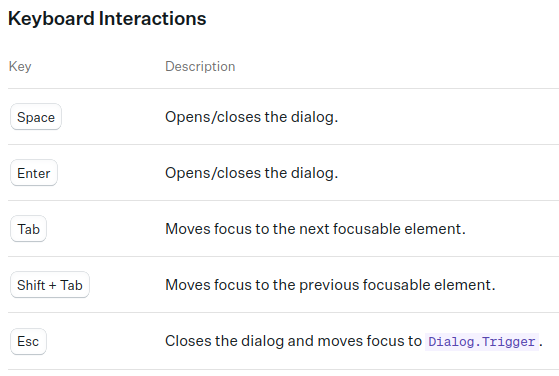
\includegraphics[width=0.75\textwidth]{Figures/radix_dialog_keyboard.png}
\decoRule
\caption[Dialog Accessability Dokumenation]{Radix UI Dialog Accessability Dokumenation}
\label{fig:radix_dialog_keyboard}
\end{figure}

\subsection{CmdK}

CmdK ist eine Open-Source-Library, die eine Komponenten basierte Accessability optimierte \textit{Combobox} bereitstellt. Eine \textit{Combobox} ist eine Kombination aus einem \textit{Input} und einer \textit{Dropdown} Liste. Diese wird inzwischen häufig auf Webseiten/Tools wie GitHub, Linear und TailwindCSS (siehe Abbildungen \ref{fig:cmdk_github}, \ref{fig:cmdk_linear}, \ref{fig:cmdk_tailwindcss}) genutzt um zum einen eine Suchfunktion zu implementieren oder um eine Liste von Aktionen / Optionen anzuzeigen. Die Tastenkombinationen für solche Funktionen sind von System zu System unterschiedlich. Zum Beispiel stellt macOS unter \emph{Cmd + Leertaste} eine Globale Such/Kommandofunktion zur Verfügung auf Webseiten wird meist eher \emph{Cmd + K} (macOs) oder \emph{Ctrl + K} (Windows) verwendet. Eine weitere Variante ist das einfache drücken von ``/``. Dies ist aber z.B. auf dem deutschen QWERTZ-Tastatur Layout nicht direkt möglich.

\begin{figure}[th]
    \centering
    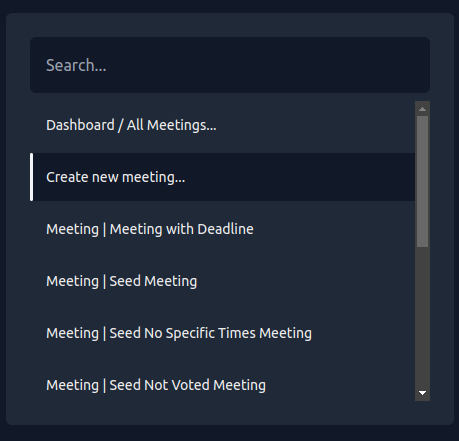
\includegraphics[width=0.6\textwidth]{Figures/turbomeet_cmdk.png}
    \decoRule
    \caption[Turbomeet Kombobox]{Turbomeet Kombobox für Seitennavigation/Suche}
    \label{fig:turbomeet_cmdk}
\end{figure}

Die Implementierung in Turbomeet (siehe Abbildung \ref{fig:turbomeet_cmdk}) lässt quasi alle oben genannten Kombinationen zu um Systemunabhängig für verschiedene Nutzer einfach bedienbar zu sein.

Zur Auswahl stehen unter anderem die Hauptseite wie das Dashboard, Nutzerprofil oder die Datenschutzerklärung, dazu werden außerdem Direkt-Verlinkungen zu den eigenen Meetings mit angezeigt. Des Weiteren werden Funktionen wie das erstellen von neuen Meetings oder das wechseln des Themes direkt ansprechbar gemacht.

Diese Funktionalität ist auch für die Accessability ein sehr interessantes Feature. So kann z.B. ein Screenreader Nutzer die Kombobox öffnen und die verfügbaren Optionen durchlesen. Wenn ein Nutzer eine Seite bereits kennt, kann er durch die Suche direkt zu dieser springen ohne erst durch verschlungene Navigationen und Submenüs zu navigieren. Hierbei sind aber auch wieder die Entwickler gefragt um die Suchbegriffe so zu wählen, dass sie für den Nutzer intuitiv sind. Dies kann z.B. auch durch eine duplizierte Navigation unter verschiedenen Begriffen erreicht werden. Dies wäre in einer normalen Navigation nicht möglich, da die Navigation dann zu unübersichtlich wird.

Ein großer Vorteil von CmdK ist, dass es für die Dialog/Popover Implementierung Radix-UI als Basis nutzt. Dies ist für Turbomeet von Vorteil, da Radix sowieso genutzt und geladen wird und somit keine zusätzlichen Abhängigkeiten hinzugefügt werden müssen und darauf vertraut werden kann, dass die Accessability Features von Radix auch in CmdK implementiert sind.

\section{Analyse}

\subsection{Lighthouse}

Da Lighthouse eines der am einfachsten und schnellsten Tools für eine Analyse auch während der Entwicklung ist habe ich mich vorrangig darauf gestützt. Die Ergebnisse wahren hier auch immer recht gut und ich konnte so schnell die kleinen Dinge verbessern, die noch nicht optimal waren. Die Ergebnisse von einem Zwischenstand sind in der folgenden Abbildung \ref{fig:lighthouse_desktop_1} zu sehen. Die kompletten Berichte sind als PDF verfügbar, aber nicht im Anhang eingebunden, da diese über 100 Seiten umfassen. Daher sind sie über den folgenden Link abrufbar: \href{https://github.com/TKSpectro/web-interaction-documentation/tree/master/Reports}{GitHub.com/TKSpectro/web-interaction-documentation}.

\begin{figure}[th]
    \centering
    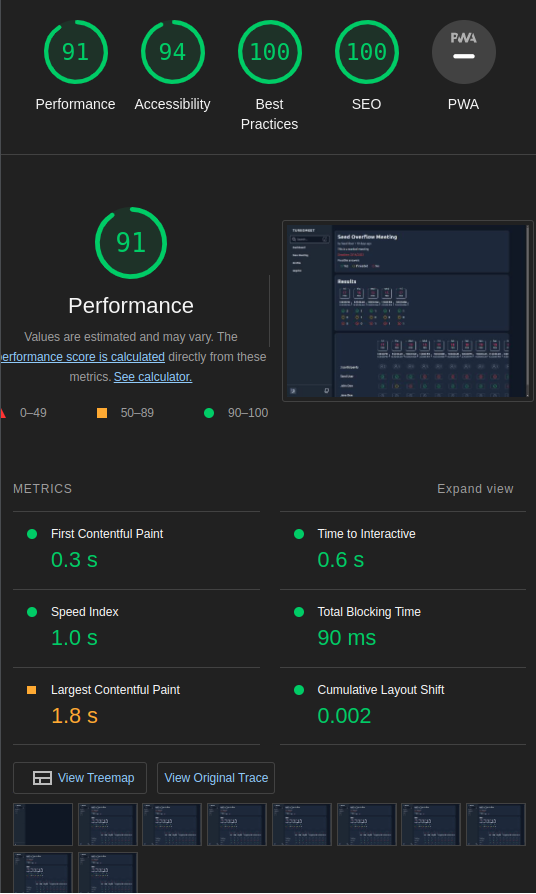
\includegraphics[width=0.45\textwidth]{Figures/lighthouse_desktop_1.png}
    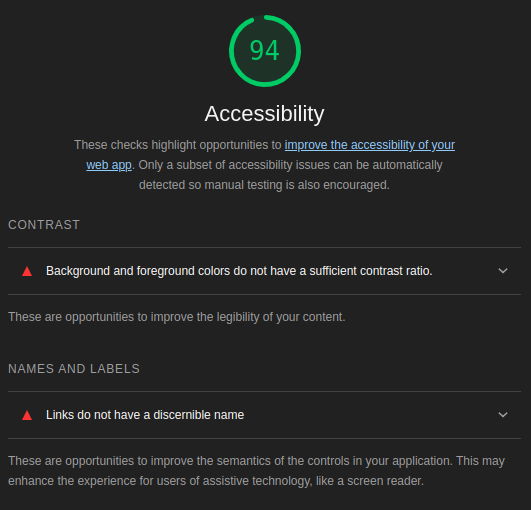
\includegraphics[width=0.45\textwidth]{Figures/lighthouse_desktop_2.png}
    \decoRule
    \caption[Turbomeet Lighthouse Bericht Desktop]{Lighthouse Bericht für Desktop}
    \label{fig:lighthouse_desktop_1}
\end{figure}

Im Bereich Accessability wurde hier z.B. darauf hingewiesen, dass die Hinter- /Vordergrund (Text) Farben zu wenig Kontrast haben und dass bei vielen Links die Beschreibungen fehlen. Als ich dann aber die Analyse noch einmal für das Mobile-Preset durchgeführt habe (siehe Abbildung \ref{fig:lighthouse_mobile_1}) 
sank die Performance von 91\% auf gerade einmal 52\%, die TTI (Time to Interactive) von 0.6s auf 6.7s und die LCP (Largest Contentful Paint) von 1.8s auf 9.2s.

\begin{figure}[th]
    \centering
    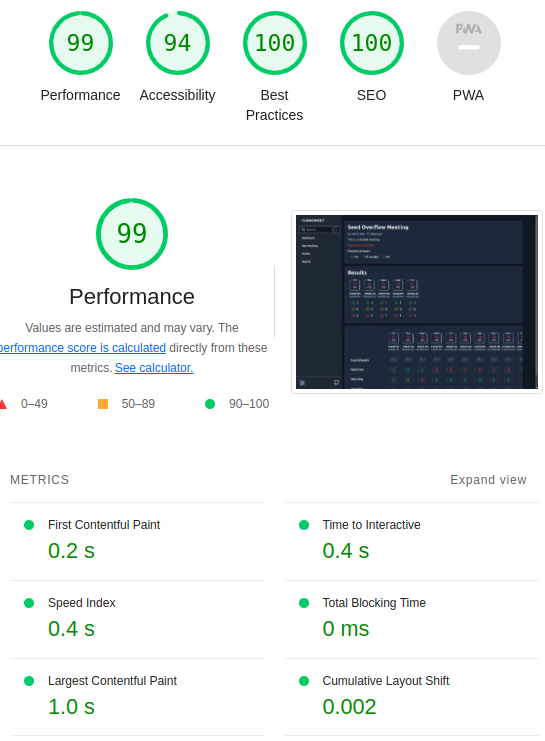
\includegraphics[width=0.45\textwidth]{Figures/lighthouse_desktop_4.png}
    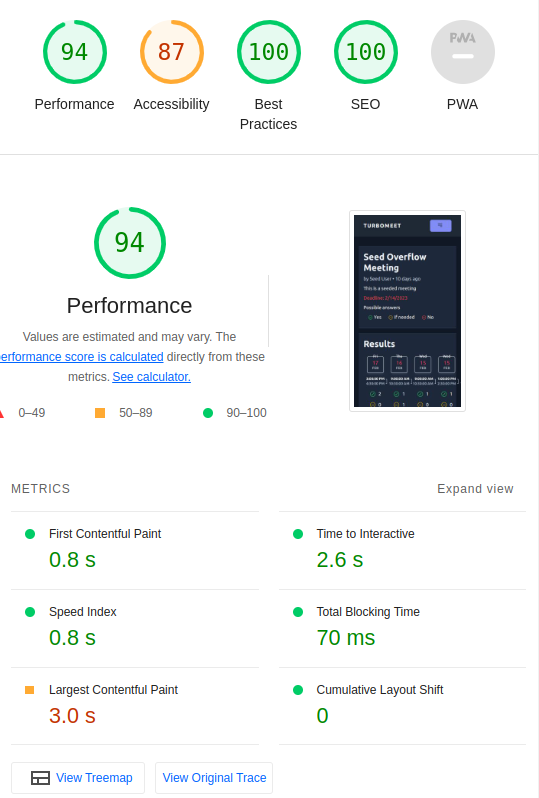
\includegraphics[width=0.45\textwidth]{Figures/lighthouse_mobile_2.png}
    \decoRule
    \caption[Turbomeet Lighthouse Bericht Chromium]{Lighthouse Bericht Chromium (links: Desktop, rechts: Mobile)}
    \label{fig:lighthouse_mobile_2}
\end{figure}

Glücklicherweise gab Lighthouse aber auch direkt den richtigen Tipp, welchen bereits im Kapitel \ref{sec:a11yToolsLighthouse} beschrieben wurde. Durch das Testen in meinem normalen Browser waren verschiedene Erweiterungen aktiv, welche sich in den Render Prozess von React einhängen um so während der Entwicklung States und ähnliche Dinge auszulesen. Aus diesem Grund schlägt Lighhouse hier vor, die Erweiterungen zu deaktivieren oder auf einen Inkognito Modus umzusteigen. Mit einem erneuten Test in einem cleanen Chromium Browser wurde nun wieder eine sehr gute Performance erreicht, jedoch sank die Accessability trotzdem noch auf 87\%. Dies liegt daran, dass Lighthouse in der Mobilen Variante alle Links als Buttons interpretiert und somit die Beschreibungen für die Button (Links) verlangt. Anscheinend weißt Lighthouse diesem dann auch mehr Gewicht zu als in der Desktop Variante. Dies ist aber auch kein Problem, da die Beschreibungen für die Links sowieso noch fehlen und somit schnell nachgeholt werden können.

Daraus lässt sich mitnehmen, immer beide Varianten zu testen, da die Ergebnisse sich unterscheiden können und auch verschiedene Optimierungen für Desktop und Mobile getroffen werden müssen. 

Die Punkte SEO und Best Practices wurden hierbei in beiden Varianten mit 100\% bewertet und dies ohne das extra Aufwände dafür getätigt werden mussten. Dies liegt daran, dass Turbomeet auf einen Technologie Stack aufbaut, welcher zum einen Next.js und das SSR Feature nutzt, wodurch die Seiten bereits vor dem Laden der Seite, auf dem Server, gerendert werden und somit auch schon für Suchmaschinen verfügbar sind (Crawlable für Google Bots). Zum anderen wird TypeScript genutzt, durch welches die neusten Features von JavaScript auch in älteren Browser polyfilled und deprecated APIs vermieden werden und somit eine sehr gute Performance erreicht wird.
\chapter{Fazit}
\label{Conclusion}


%----------------------------------------------------------------------------------------
%	THESIS CONTENT - APPENDICES
%----------------------------------------------------------------------------------------

\appendix % Cue to tell LaTeX that the following "chapters" are Appendices

% Include the appendices of the thesis as separate files from the Appendices folder
% Uncomment the lines as you write the Appendices

\chapter{Abbildungen}
\label{appendix:images}

\begin{figure}[th]
    \centering
    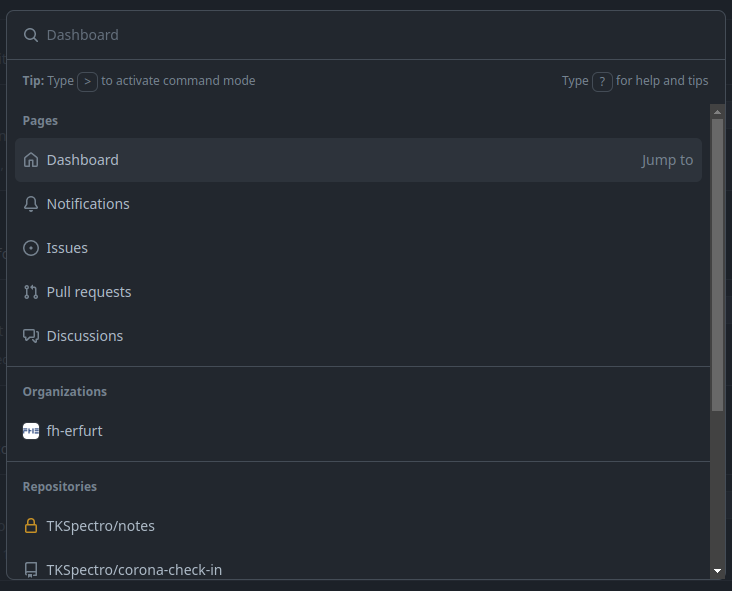
\includegraphics[width=0.9\textwidth]{Figures/cmdk_github.png}
    \decoRule
    \caption[GitHub Kombobox]{GitHub Kombobox}
    \label{fig:cmdk_github}
\end{figure}

\begin{figure}[th]
    \centering
    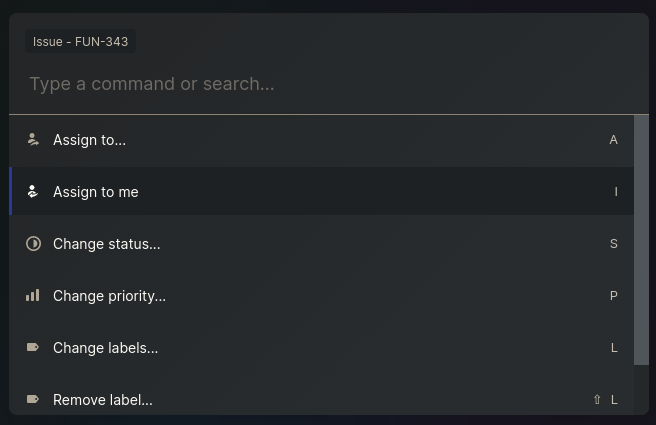
\includegraphics[width=0.9\textwidth]{Figures/cmdk_linear.png}
    \decoRule
    \caption[Linear Kombobox]{Linear Kombobox}
    \label{fig:cmdk_linear}
\end{figure}

\begin{figure}[th]
    \centering
    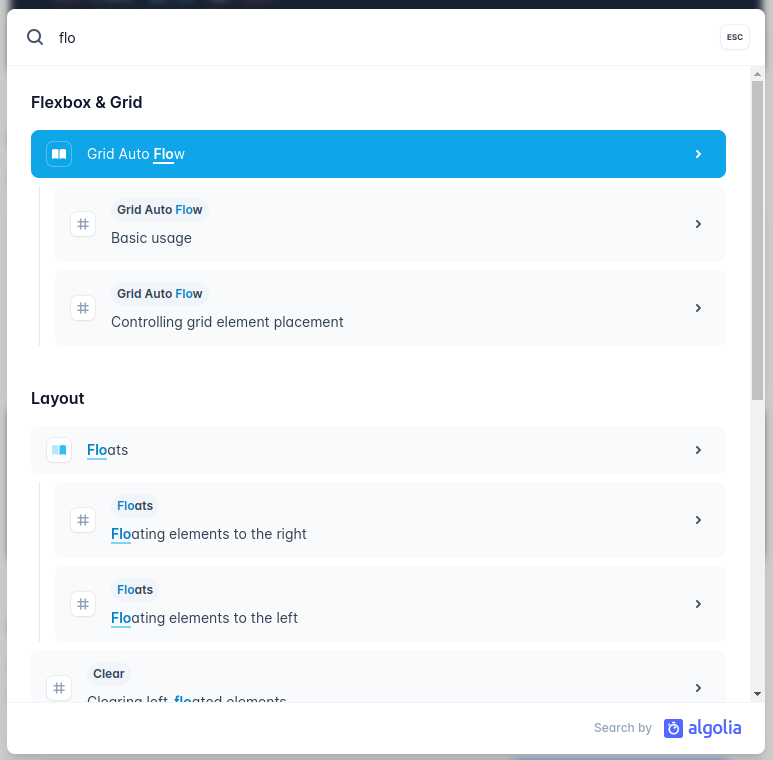
\includegraphics[width=0.9\textwidth]{Figures/cmdk_tailwindcss.png}
    \decoRule
    \caption[TailwindCSS Kombobox]{TailwindCSS Kombobox}
    \label{fig:cmdk_tailwindcss}
\end{figure}

\begin{figure}[th]
    \centering
    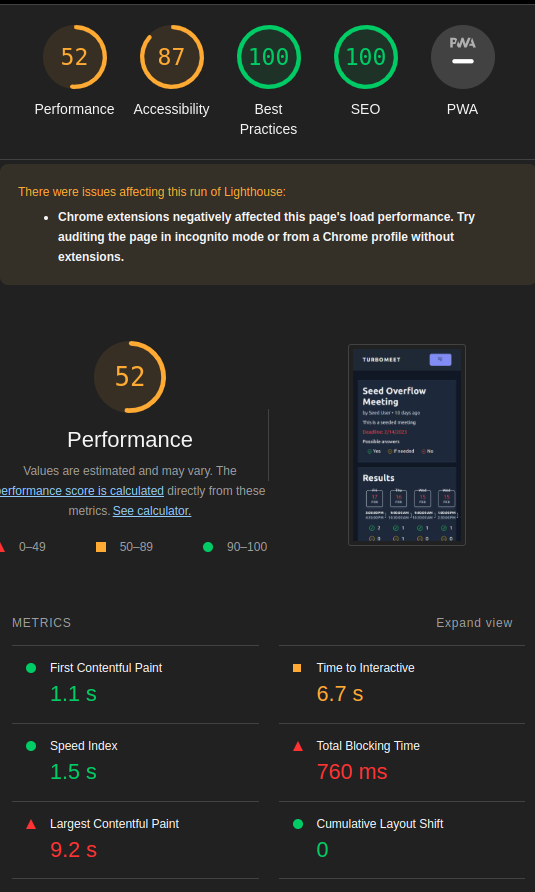
\includegraphics[width=0.45\textwidth]{Figures/lighthouse_mobile_1.png}
    \decoRule
    \caption[Turbomeet Lighthouse Bericht Mobile]{Lighthouse Bericht für Mobile Zwischenstand}
    \label{fig:lighthouse_mobile_1}
\end{figure}
\chapter{Quellcode}
\label{appendix:sourcecode}

\lstinputlisting[caption=TailwindCSS Konfiguration, label=listing:tailwindcss_config]{Listings/tailwind.config.cjs}
%\include{Appendices/AppendixB}
%\include{Appendices/AppendixC}

%----------------------------------------------------------------------------------------
%	BIBLIOGRAPHY
%----------------------------------------------------------------------------------------

\printbibliography[heading=bibintoc]

%----------------------------------------------------------------------------------------

\end{document}  
